\documentclass[12pt]{article}
\usepackage[utf8]{inputenc}
\usepackage[T1]{fontenc}
\usepackage[a4paper,left=2cm,right=2cm,top=2cm,bottom=2cm]{geometry}
\usepackage[frenchb]{babel}
\usepackage{libertine}
 \usepackage{setspace}
\usepackage[pdftex]{graphicx}
\setlength{\parindent}{4em}
\setlength{\parskip}{1em}
\newcommand{\hsp}{\hspace{20pt}}
\newcommand{\HRule}{\rule{\linewidth}{0.5mm}}

\doublespacing
\begin{document}
	
\begin{titlepage}
  \begin{sffamily}
  \begin{center}
    
    
\includegraphics[scale=0.5]{./images/unicaenLogo.png}

    \textsc{\LARGE 2ème Licence Informatique }\\[2cm]
    \textsc{\Large Groupe 2B }\\[1.5cm]

    \textsc{\Large RAPPORT }\\[1.5cm]

    % Titre
    \HRule \\[0.4cm]
    { \huge \bfseries Éditeur de livres dont vous êtes le héros\\[0.4cm] }

    \HRule \\[2cm]
    
    

    % Auteurs
    \begin{minipage}{0.4\textwidth}
      \begin{center}\large
      	AUTEURS:\\
      	WAKARY DOUCOURE\\FAICAL SID AHMED RAHMANI\\MATEJ TRPKOVSKI\\MICHEL KAZADI KALALA
      \end{center}
    \end{minipage}

    \vfill    
    {\large 20 Avril 2021}

  \end{center}
  \end{sffamily}
\end{titlepage}

	\thispagestyle{empty}
	\setcounter{page}{0}
  	\newpage
  	\tableofcontents
  	\newpage
  	

  	
	\section*{Introduction}
	\addcontentsline{toc}{section}{\protect\numberline{}Introduction}%
	La programmation informatique notamment celle Orientée Objet a une place très importante au sein du cursus informatique. C'est pourquoi pour mettre en pratique nos connaissances et nous développer  en Java, l'unité d'enseignement Conception Logicielle nous propose divers projets sur lesquels travailler.
	\par Par groupes d'au plus 4 personnes, il nous a été demandé de réaliser une application
	 parmi plusieurs proposées, notre choix s'est porté sur \textit{"l'éditeur de Livre dont vous êtes le héros"} dont l'énoncé est le suivant:\\
	<<: Les livres dont vous êtes le héros (ou LDVEH) sont des jeux de rôles en solitaire dont la
		narration est décomposées en paragraphes, dispersés dans le livre. Des liens, en fonction des 			choix du lecteurs, permettent d’aller d’un paragraphe à l’autre. Dans un premier temps, il s’agira de
	développer un éditeur de texte qui maintienne le graphe du jeu et qui puisse réorganiser
	aléatoirement le livre. L’affichage de la ou les solutions (paragraphe devant être traversés pour
	gagner) devront être calculées ainsi que la difficulté du jeu (proportions de solutions au regard des
	chemins possibles). Dans un second temps, il s’agira d’ajouter un système de rencontres et de
	combat, ainsi que la gestion d’objets ou d’indices qui peuvent être nécessaire pour gagner. Enfin,
	un mode lecture permettant de jouer au LDVEH pourra être implanté.>>
	\par La réalisation de ce projet se base principalement sur l'éditeur de Texte qui permettra de:
	\begin{itemize}
		\item Construire un Livre (Création des paragraphes [noeuds]\footnote{Tout au long de ce rapport, on utilisera le mot noeud pour désigner un paragraphe et vis versa.} qui constituent un Livre).
		\item Jouer à un Livre ( Jouer une histoire \footnote{On utilisera le mot histoire pour désigner un livre et vis versa.} déjà créée   ).
	\end{itemize}
	\newpage
	
		
	

	\section{Organisation du projet}
	    \subsection{Répartition des tâches}
	   Afin de produire le jeu dans la limite du temps donné, nous avons dû élaborer un plan de travail, ainsi que répartir les tâches. Nous avons donc décidé dans un premier temps , de nous séparer en binôme . Michel et Faical ont d'abord travaillé sur l'implémentation du graphe\footnote{un graphe permet de mettre en relation plusieurs noeuds .}  et au même moment wakary et Matej essayaient de trouver une façon optimale de créer l'interface graphique de base  (L'éditeur de Texte). \\Malgré le plan de travail établi , la conception de ce dernier (l'interface graphique) a demandé bien plus de temps que prévu, notamment dû au fait que wakary et Matej dévraient utiliser Java Swing\footnote{bibliothèque graphique en Java}, qu'ils ne maîtrisaient pas encore en ce moment-là .Ainsi l'implémentation du système de graphe étant terminée, Michel et Faical ont pu commencer en parallèle des recherches sur la création de l'interface graphique mais aussi sur le système des sauvegardes des livres (histoires) qui interviendront après leurs créations. Dans un second temps, Michel et Faical se sont aussi occupés de l'implementation du système de construction d'un Livre et du système pour Jouer un Livre . 
        \newpage
	    \subsection{Architecture du programme}
	    Concernant l'architecture du programme, nous avons opté pour 5 packages:\\
	\textbf{graphs}: qui contient les classes relatives au système de graphe.\\
	Le package graphs est composé de classes  :
	\begin{itemize}
		\item \textbf{\textit{Noeud}} : classe de base pour créer un Noeud (paragraphe dans un Livre). Elle contient des attributs : description (énoncé du texte contenu dans un paragraphe) , question  et identifiant (id unique).
		 \item \textbf{\textit{Réponse}}: une réponse est constituée d'un texte ainsi qu'une référence vers le paragraphe (Noeud) de destination.
	\end{itemize}
	\textbf{createStory}: qui comme son nom l'indique permet de créer une histoire (Livre) sur une interface graphique \\	Ce package est composé de :
	\begin{itemize}
		\item \textbf{\textit{AddReponse}} : cette classe permet d'ajouter une réponse à un Noeud .
		 \item \textbf{\textit{EditReponse }}: Elle permet de modifier une réponse , en changeant son noeud de destination ou son texte.
		  \item \textbf{\textit{CreateBookPage }}: La classe CreateBookPage  contient toutes les fonctionnalités(les zones de texte, les boutons etc)  qui permettent de créer une histoire.
		  \item \textbf{\textit{ManageBook }}: Cette classe s'occupe de la gestion de toutes les autres classes de ce package.
	\end{itemize}
	\textbf{playStory}: Il permet de jouer une histoire créée au préalable. \\
	Le package playStory est composé de :
	\begin{itemize}
		\item \textbf{\textit{GamePage}} : cette classe contient toutes les fonctionnalités qui permettent de jouer à une histoire.
		 \item \textbf{\textit{playBookPage }}: classe qui permet de choisir une histoire pour la jouer.
	\end{itemize}
	\textbf{welcome}: package principal qui permet l'execution du programme. \\
	Il est composé de :
	\begin{itemize}
		\item \textbf{\textit{StartPage}} : classe de demarrage et page d'acceuil du programme.
		 \item \textbf{\textit{Main }}: classe qui permet d'exécuter le programme .
	\end{itemize}
	\textbf{tools}: qui est constitué de toutes les classes  considérées comme étant des outils importants pour le bon déroulement du programme.	\\ Ce package est constitué de :
	\begin{itemize} 
	 \item \textbf{\textit{ImagePanel}} : cette classe sert à l'affichage des images utilisées sur l'interface graphique.		 \item \textbf{\textit{SettingsPage}}: classe qui permet le paramétrage de l'interface graphique (font Size ,font Color, fontType ).
	  \item \textbf{\textit{XmlBackup}}: classe qui s'occupe de la sauvegarde d'une histoire.
	\end{itemize}
	
	
	\subsection{Diagramme des packages}
	
		\begin{center}
		\begin{verse}
		    \begin{center}
		       \textbf{Diagramme du Package graphs} 
		    \end{center}
		\end{verse} 
			\newcommand{\umlscale}{0.4}
			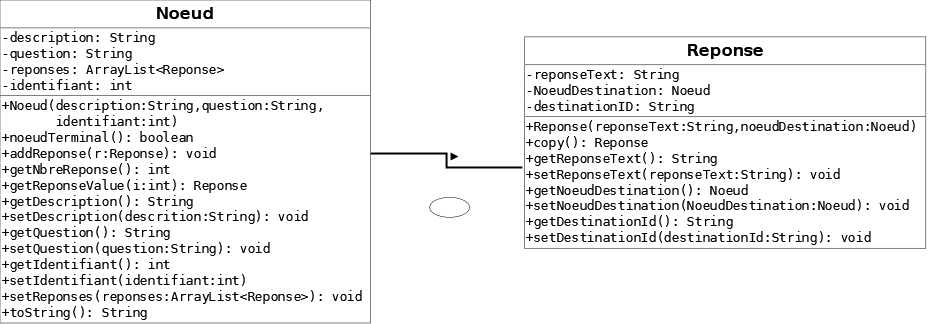
\includegraphics[scale=\umlscale]{./images/packageGraphs.png}
		\end{center}
	

	    \begin{center}
		\begin{verse}
		    \begin{center}
		       \textbf{Diagramme du Package playStory} 
		    \end{center}
		\end{verse} 
			\newcommand{\umlscale}{0.4}
			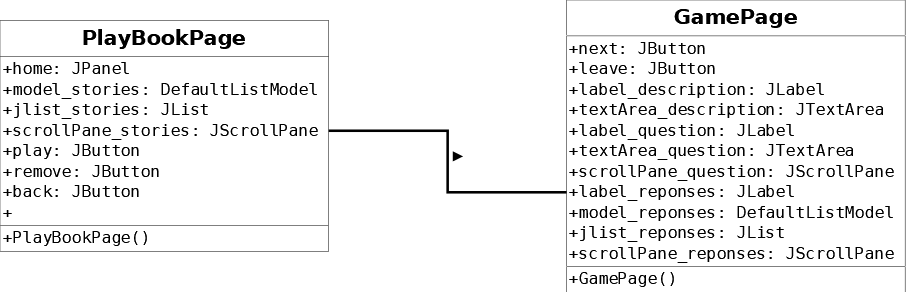
\includegraphics[scale=\umlscale]{./images/packagePlayStory.png}
		\end{center}
	
	
		\begin{center}
		\begin{verse}
		    \begin{center}
		       \textbf{Diagramme du Package createStory} 
		    \end{center}
		\end{verse}
			\newcommand{\umlscale}{0.4}
			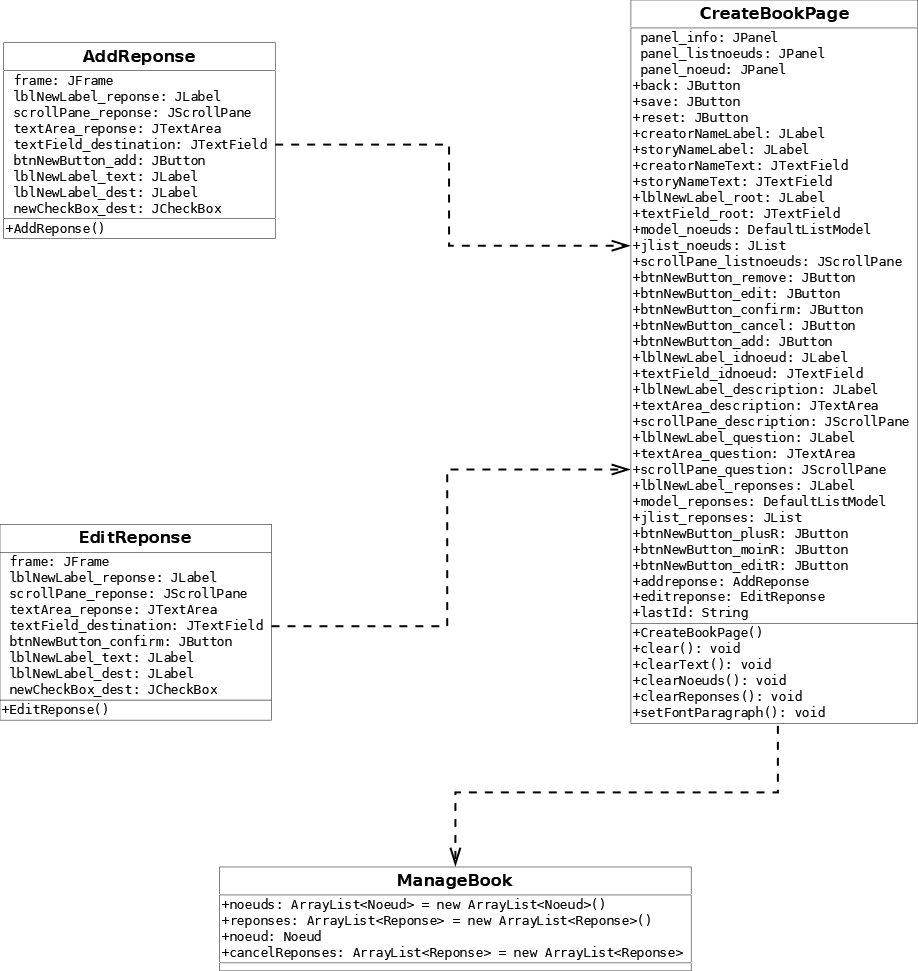
\includegraphics[scale=\umlscale]{./images/packageCreateStory.png}
		\end{center}
	    \newpage
		\begin{center}
		\begin{verse}
		    \begin{center}
		       \textbf{Diagramme du Package tools} 
		    \end{center}
		\end{verse}
			\newcommand{\umlscale}{0.4}
			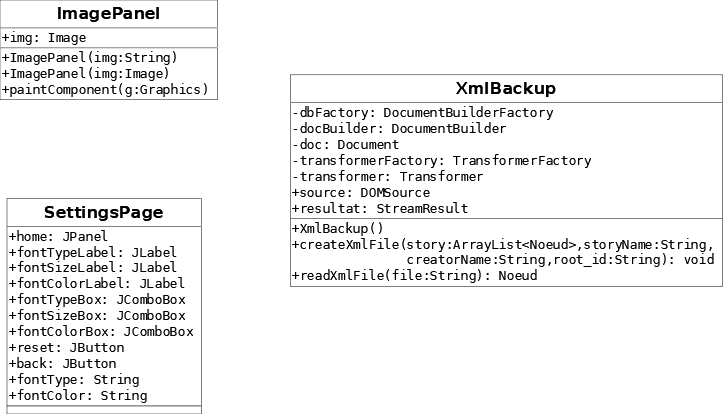
\includegraphics[scale=\umlscale]{./images/packageTools.png}
		\end{center}
		\begin{center}
		\begin{verse}
		    \begin{center}
		       \textbf{Diagramme du Package welcome} 
		    \end{center}
		\end{verse}
			\newcommand{\umlscale}{0.4}
			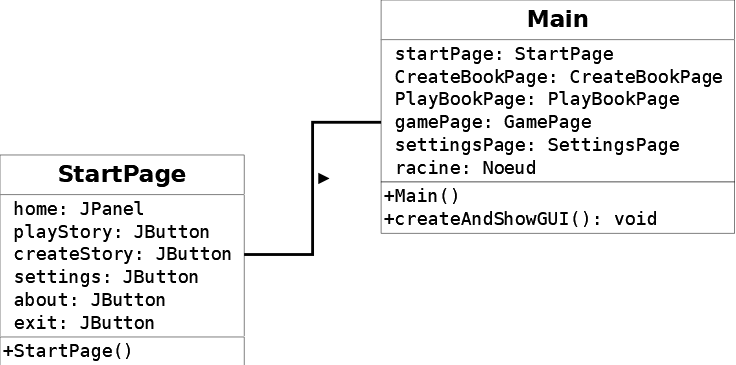
\includegraphics[scale=\umlscale]{./images/packageWelcome.png}
		\end{center}
		
	    \newpage
		\begin{center}
		\begin{verse}
		    \begin{center}
		       \textbf{Diagramme des Packages} 
		    \end{center}
		\end{verse}
			\newcommand{\umlscale}{0.4}
			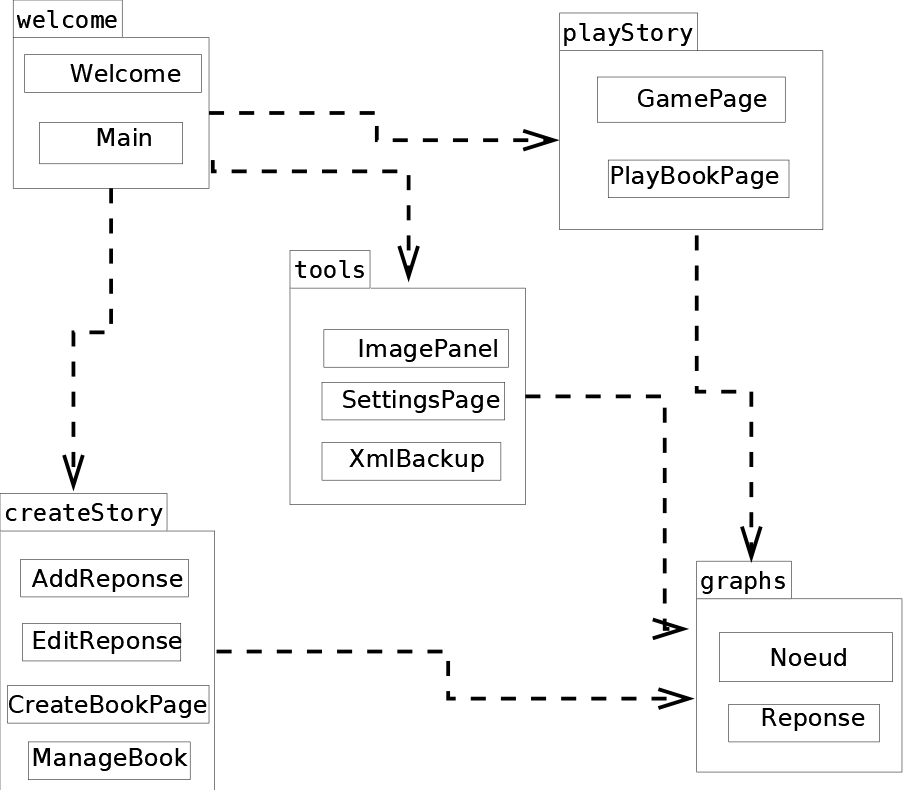
\includegraphics[scale=\umlscale]{./images/packageDiagram.png}
		\end{center}
	
	\newpage
	\section{Elements techniques}
	\subsection{Système de sauvegarde}
	L'implémentation de notre projet (Éditeur de livres dont vous êtes le héros) nécessitait un système de sauvegarde pour converser les livres déjà crées, un peu comme une bibliothèque où l'on trouve un ensemble de livres. Nous avons réfléchi à mille et une façon d'implémenter ce système  et nous avons finalement décidé de  faire la sauvegarde en utilisant XML(L'extensible Markup Langage)\footnote{Langage de balisage extensible}. Ce système comprend deux parties:
	\begin{itemize}
		\item \textit{la transformation d'une liste de noeuds en Chaîne de Caractères (String) et sa sauvegarde dans un fichier.}
		\item \textit{la transformation d'un fichier (ensemble de Chaîne de Caractères) en liste des noeuds}.\\
	\end{itemize}
    \textbf{1. From Node to String}\\
    Pour pouvoir facilement transformer une liste de noeuds en chaîne de Caractères, nous avons créé une fonction qui prend en paramètre: la liste des noeuds, le titre du livre, l'auteur du livre et le noeud racine.\footnote{noeud considéré comme étant le début du livre. }. En utilisant XML, nous avons stocké tous ces éléments dans des balises. Vu qu'il s'agit d'une liste de noeuds, nous avons utilisé une boucle For pour parcourir la liste entière et pour chaque noeud, on parcourt toutes ses réponses. À la fin de chaque transformation, un fichier contenant cette transformation est créé puis conservé. \\\\
    \textbf{2. From String to Node}\\
	La transformation d'un fichier contenant des chaînes de Caractères en liste de noeuds, est une opération inverse à la première. Pour y arriver, nous avons créé une méthode qui prend en paramètre le fichier à transformer, dans le corps de cette méthode, nous avons initialisé une liste de noeud ainsi qu'un noeud racine, grâce à XML, nous avons pu récupérer la valeur du noeud racine dans le fichier et à partir du noeud racine, nous avons fait une opération récursive pour pouvoir récupérer la liste des noeuds ainsi que leurs réponses respectives.
    \subsection{Système de Création d'un Livre}
    Nous avons créé une interface graphique permettant de créer un Livre  . Cette interface contient 3 zones principales :
    \begin{itemize}
		\item \textit{Zone d'informations}.
		\item \textit{Zone de création d'un paragraphe}.
		\item \textit{Zone liste des noeuds}.\\
	\end{itemize}
	 \textbf{1. Zone d'informations}\\
	 Cette zone permet de remplir les informations importantes lors de la création d'un livre, notamment le nom de l'auteur ainsi que le titre du livre.\\ \textbf{2. Zone de création d'un paragraphe}\\ Cette zone permet de créer un paragraphe.\\ Elle est constituée de :
	 \begin{itemize}
		\item {un champs de texte permettant de remplir l'identifiant du paragrahe}.
		\item {un champs de texte permettant de remplir la description du paragrahe}.
		\item {un champs de texte permettant de remplir la question du paragrahe}.
		\item {un champs de texte permettant de remplir les reponses du paragrahe}\\
	\end{itemize}
    \textbf{3. Zone liste de noeuds}\\	 
   Cette zone comprend la liste de tous les noeuds déjà créés, Elle comprend aussi les boutons ;
   \begin{itemize}
    \item {remove : pour supprimer un noeud}.
    \item {edit : pour modifier un noeud}
  \end{itemize} 
  \newpage
  \section{Conclusion}
  \subsection{Objectifs remplis ?}
  Réaliser un travail de groupe , nécessite une organisation, une répartition des tâches, une gestion du temps. Nous avons eu un peu de mal à mettre en place toutes ces recommandations pour mener à bien notre projet à cause de la situation sanitaire actuelle et au fait que l'intégralité du projet a été réalisée à distance.\\  Néanmoins, nous avons presque tout implémenté en ce qui concerne les fonctions de base de notre programme. En commençant par implémenter le système de graphes, qui permet de mettre en relation l'ensemble des noeuds, ensuite par la création d'un éditeur de texte, qui permet de créer une histoire et enfin par la réalisation d'une interface graphique qui permet de jouer à une histoire.
  \subsection{Améliorations possibles}
  Concernant les améliorations possibles, on aurait pu ajouter : l'affichage des solutions possibles (paragraphe devant être traversé pour gagner), un système de rencontres et de combat ainsi que la gestion d'objets ou d'indices qui peuvent être nécessaire pour gagner.
  \subsection{Leçons retenues}
  Tout au long de notre projet, nous avons retenu plusieurs leçons : la nécessité d'une bonne communication dans un groupe de travail, la gestion du temps, l'importance d'une bonne répartition des tâches etc.\\ Qu'à cela ne tienne, la réalisation de ce projet a été une très belle expérience pour nous, ça nous a permis de mettre en pratique les notions de programmation orientée objet (Java) apprissent en cours.
  
    

\end{document}


